\documentclass[a4paper]{article}
\usepackage[utf8]{inputenc}
\usepackage[russian]{babel}
\usepackage{listings}
\usepackage[a4paper,margin=1.2in]{geometry}
\usepackage{indentfirst}
\usepackage{graphicx}
\usepackage{caption}
\usepackage{float}

%\setcounter{topnumber}{2}
%\setcounter{bottomnumber}{2}
%\setcounter{totalnumber}{4}
%\renewcommand{\topfraction}{0.85}
%\renewcommand{\bottomfraction}{0.85}
%\renewcommand{\textfraction}{0.15}
%\renewcommand{\floatpagefraction}{0.8}
%\renewcommand{\textfraction}{0.1}
%\setlength{\floatsep}{5pt plus 2pt minus 2pt}
%\setlength{\textfloatsep}{5pt plus 2pt minus 2pt}
%\setlength{\intextsep}{5pt plus 2pt minus 2pt}

\begin{document}

\title{Сравнение методов глобальной оптимизации на нескольких классах тестовых задач}
\author{}
\date{}
\maketitle

\section{Список алгоритмов}
\begin{itemize}
  \item Алгоритм глобального поиска (AGS)
  \item Multi Level Single Linkage (MLSL)
  \item DIRECT
  \item Locally-based DIRECT (DIRECT$l$)
  \item Dual Simulated Annealing
  \item Differential Evolution
  \item Controlled Random Search
  \item Simple
\end{itemize}

\section{Результаты на классе задач $F_{GR}$}

\begin{figure}[H]
  \center
  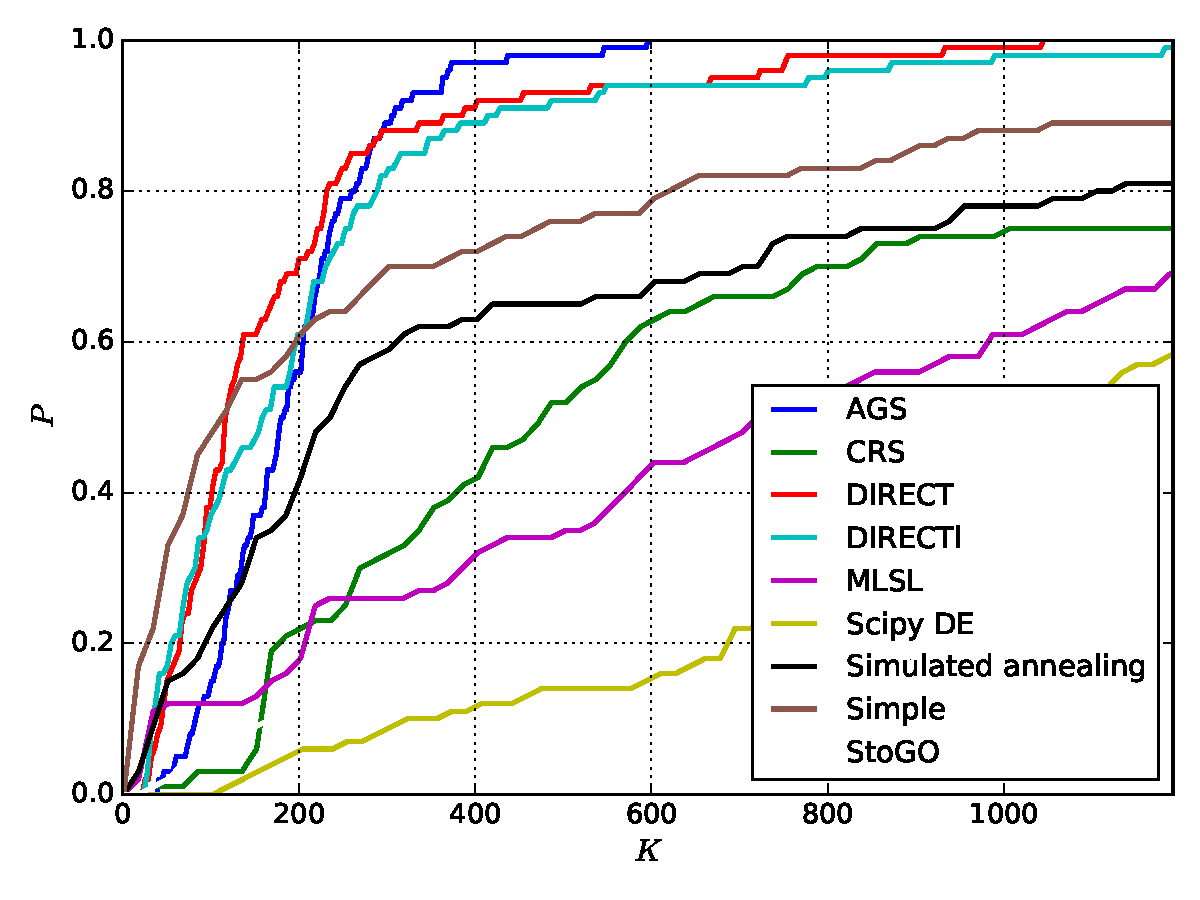
\includegraphics[width=0.95\textwidth]{../experiments/grish/cmc.pdf}
  \caption{Остановка после попадания в окрестность размера $10^{-2}$}
  \label{fig:}
\end{figure}

%table grish
\begin{tabular}{lrr}
\hline
 Метод    &   Среднее число испытаний &   Решено задач \\
\hline
 AGS      &                    193.11 &            100 \\
 CRS      &                    400.30 &             76 \\
 DIRECT   &                    182.25 &            100 \\
 DIRECTl  &                    214.92 &            100 \\
 MLSL     &                    947.18 &             97 \\
 SDA      &                    691.24 &             96 \\
 Scipy DE &                   1257.34 &             96 \\
 Simple   &                    374.12 &             97 \\
 StoGO    &                   1336.78 &             67 \\
\hline
\end{tabular}
\section{Результаты на классах задач $GKLS$ различной размерности}

\begin{figure}[H]
  \center
  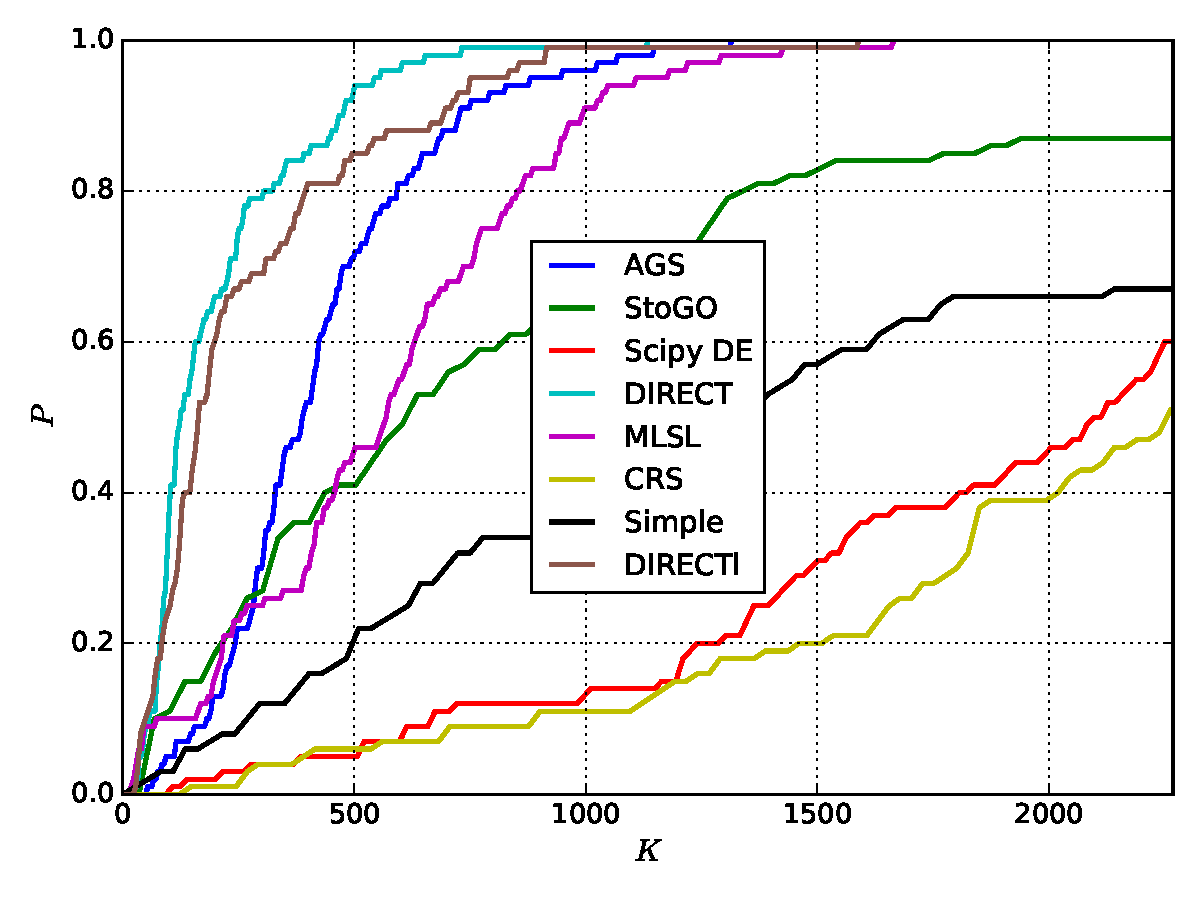
\includegraphics[width=0.95\textwidth]{../experiments/gklss2d/cmc.pdf}
  \caption{Класс GKLS Simple 2d. Остановка после попадания в окрестность размера $2\cdot10^{-2}$}
  \label{fig:}
\end{figure}

%table gklss2d
\begin{tabular}{lrr}
\hline
 Метод    &   Среднее число испытаний &   Решено задач \\
\hline
 AGS      &                    254.89 &            100 \\
 CRS      &                    510.61 &             85 \\
 DIRECT   &                    189.03 &            100 \\
 DIRECTl  &                    255.21 &            100 \\
 MLSL     &                    556.83 &            100 \\
 SDA      &                    356.30 &            100 \\
 Scipy DE &                    952.16 &             98 \\
 Simple   &                    440.63 &            100 \\
 StoGO    &                   1251.52 &             90 \\
\hline
\end{tabular}
\begin{figure}[H]
  \center
  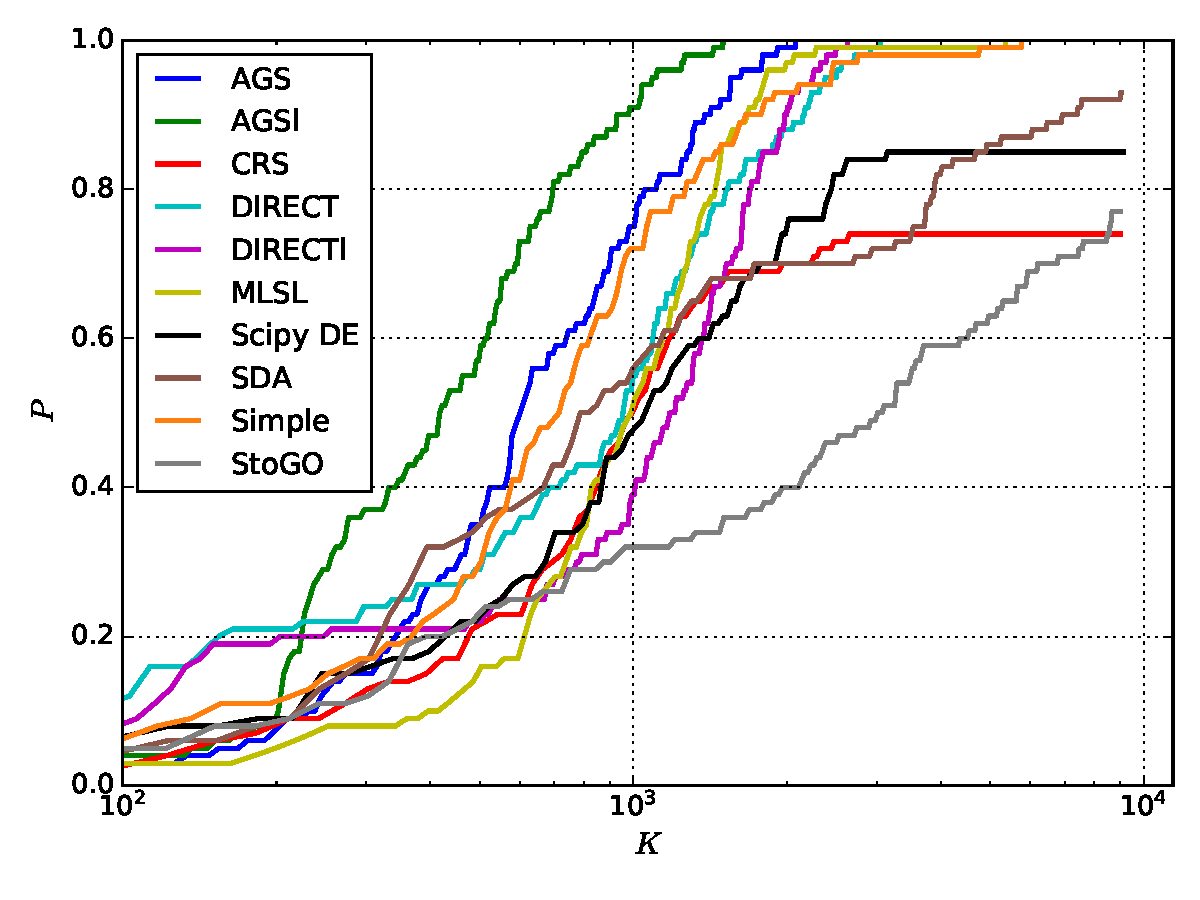
\includegraphics[width=0.95\textwidth]{../experiments/gklsh2d/cmc.pdf}
  \caption{Класс GKLS Hard 2d. Остановка после попадания в окрестность размера $2\cdot10^{-2}$}
  \label{fig:}
\end{figure}

%table gklsh2d
\begin{tabular}{lrr}
\hline
 Метод    &   Среднее число испытаний &   Решено задач \\
\hline
 AGS      &                    728.71 &            100 \\
 CRS      &                    844.74 &             74 \\
 DIRECT   &                    985.44 &            100 \\
 DIRECTl  &                   1126.65 &            100 \\
 MLSL     &                   1042.54 &            100 \\
 SDA      &                   1637.92 &             93 \\
 Scipy DE &                   1041.12 &             85 \\
 Simple   &                    898.19 &            100 \\
 StoGO    &                   2532.23 &             77 \\
\hline
\end{tabular}
\begin{figure}[H]
  \center
  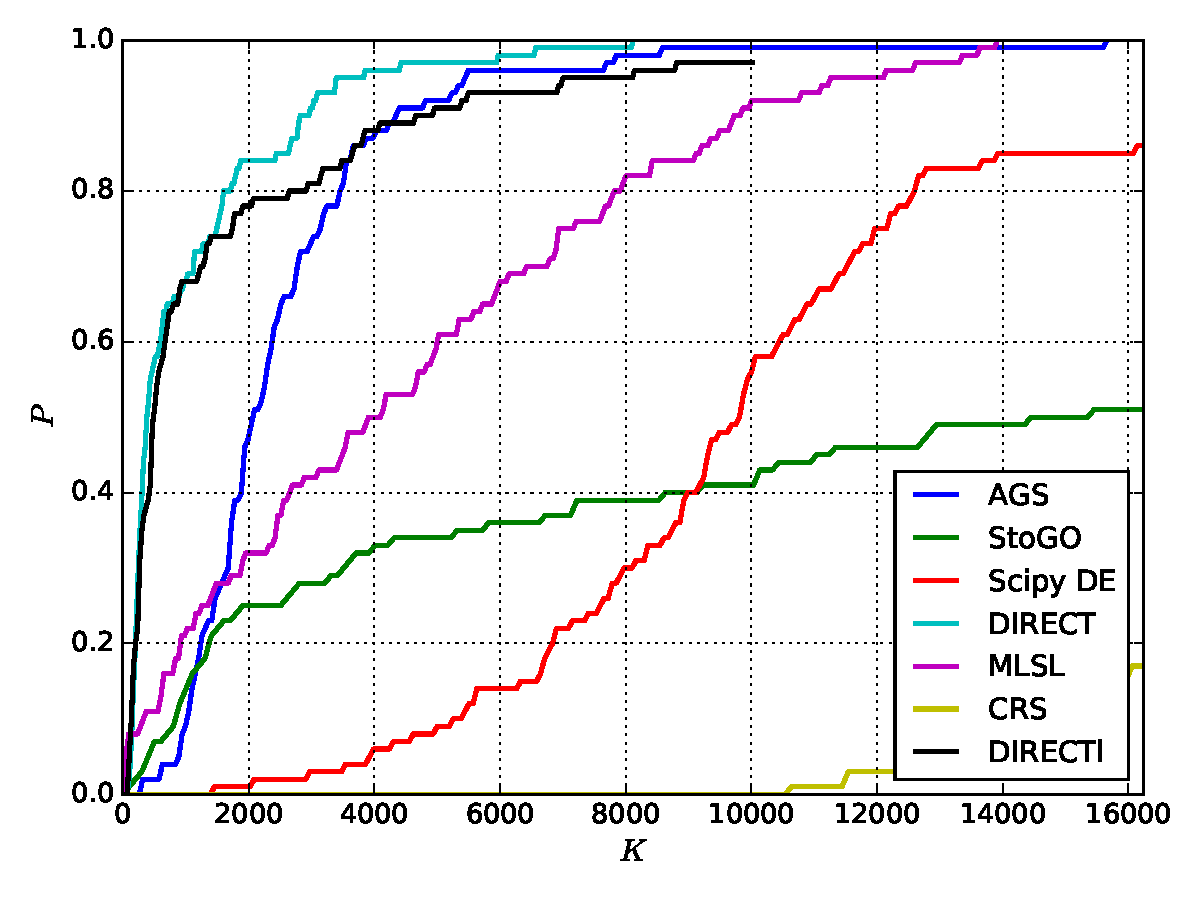
\includegraphics[width=0.95\textwidth]{../experiments/gklss3d/cmc.pdf}
  \caption{Класс GKLS Simple 3d. Остановка после попадания в окрестность размера $2\cdot10^{-2}$}
  \label{fig:}
\end{figure}

%table gklss3d
\begin{tabular}{lrr}
\hline
 Метод    &   Среднее число испытаний &   Решено задач \\
\hline
 AGS      &                   1372.13 &            100 \\
 CRS      &                   4145.81 &             75 \\
 DIRECT   &                    973.64 &            100 \\
 DIRECTl  &                   1477.79 &            100 \\
 MLSL     &                   4609.17 &            100 \\
 SDA      &                   2706.52 &             89 \\
 Scipy DE &                   5956.94 &             86 \\
 Simple   &                   7098.45 &             33 \\
 StoGO    &                   3856.11 &             44 \\
\hline
\end{tabular}
\begin{figure}[H]
  \center
  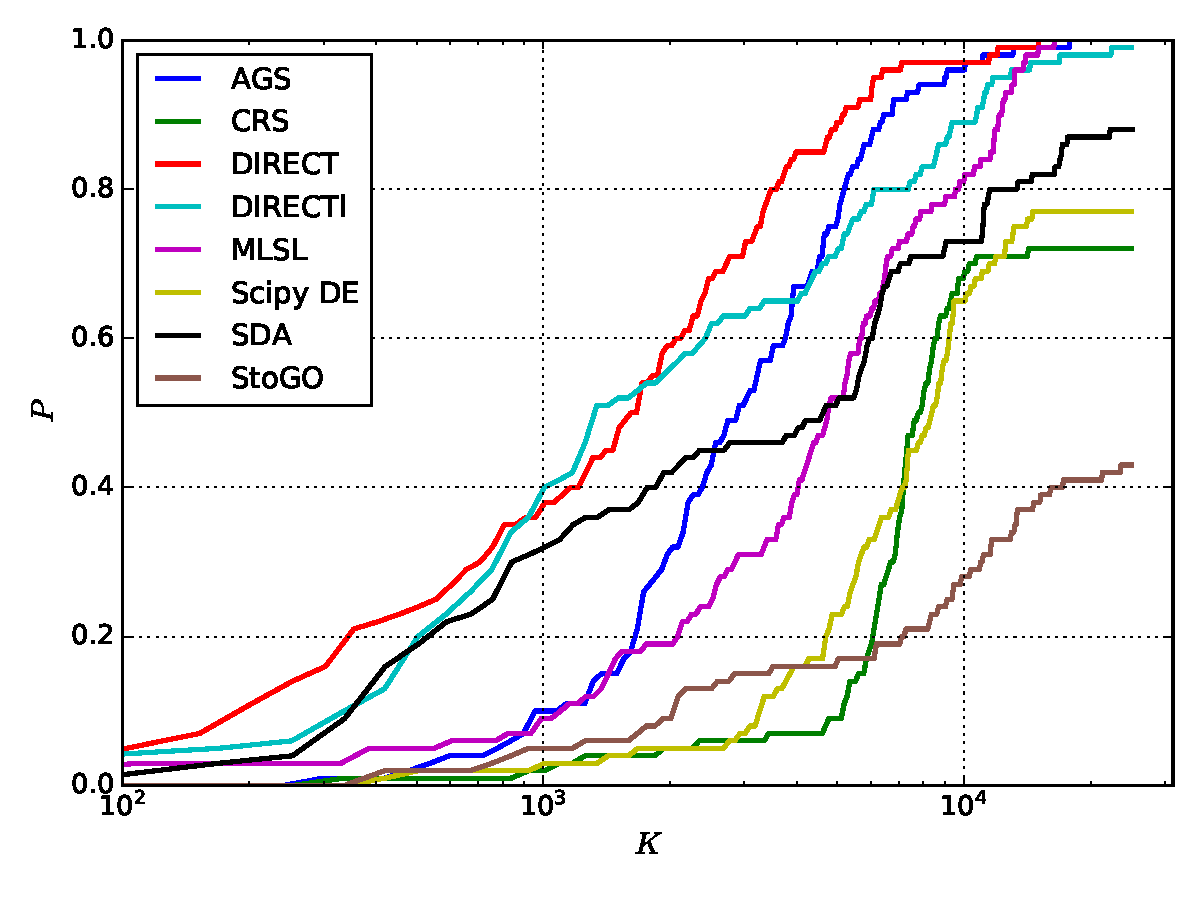
\includegraphics[width=0.95\textwidth]{../experiments/gklsh3d/cmc.pdf}
  \caption{Класс GKLS Hard 3d. Остановка после попадания в окрестность размера $2\cdot10^{-2}$}
  \label{fig:}
\end{figure}

%table gklsh3d
\begin{tabular}{lrr}
\hline
 Метод    &   Среднее число испытаний &   Решено задач \\
\hline
 AGS      &                   3636.12 &            100 \\
 CRS      &                   6786.96 &             72 \\
 DIRECT   &                   2298.74 &            100 \\
 DIRECTl  &                   3553.33 &             99 \\
 MLSL     &                   5640.10 &            100 \\
 SDA      &                   4708.43 &             88 \\
 Scipy DE &                   6914.34 &             77 \\
 StoGO    &                   7843.23 &             43 \\
\hline
\end{tabular}
\begin{figure}[H]
  \center
  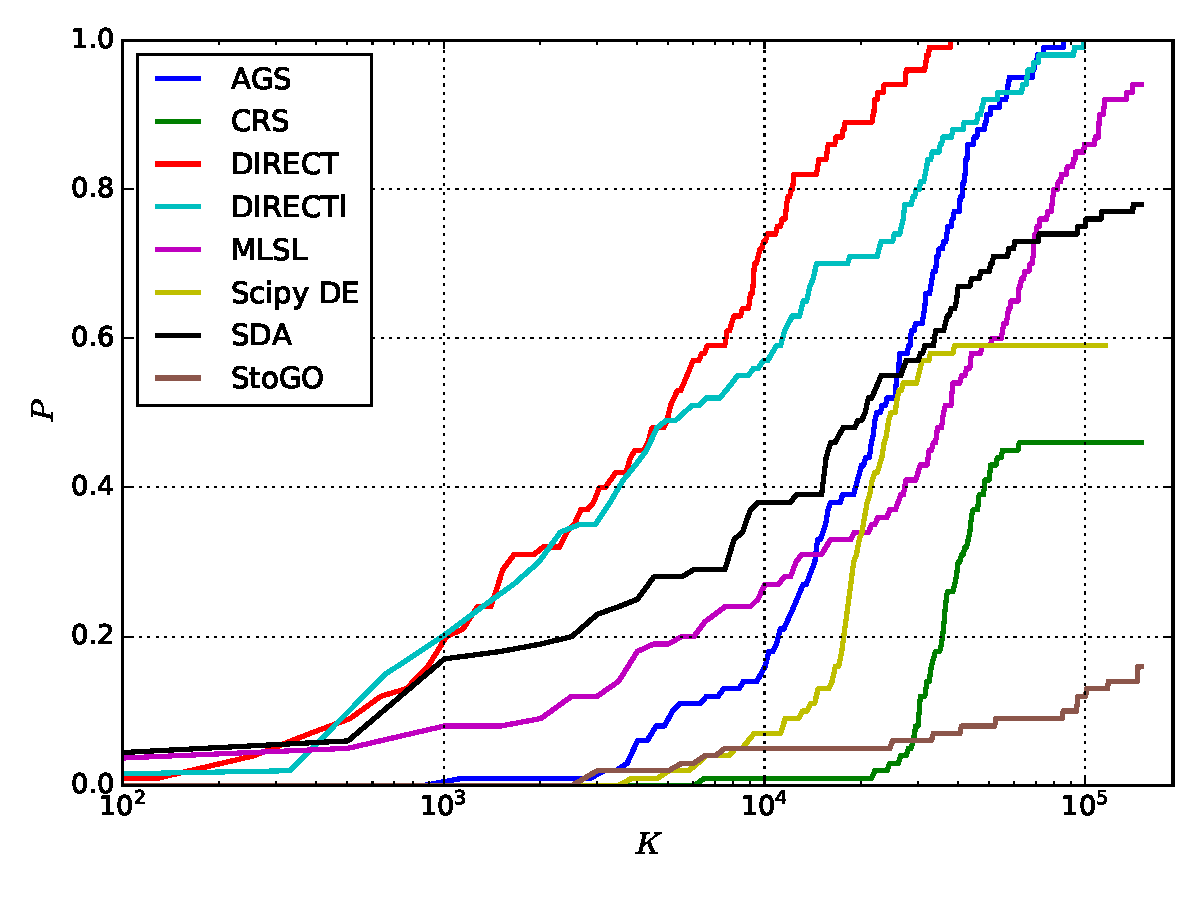
\includegraphics[width=0.95\textwidth]{../experiments/gklss4d/cmc.pdf}
  \caption{Класс GKLS Simple 4d. Остановка после попадания в окрестность размера $2\cdot10^{-2}$}
  \label{fig:}
\end{figure}

%table gklss4d
\begin{tabular}{lrr}
\hline
 Метод    &   Среднее число испытаний &   Решено задач \\
\hline
 AGS      &                  26654.07 &            100 \\
 CRS      &                  37436.76 &             46 \\
 DIRECT   &                   7824.32 &            100 \\
 DIRECTl  &                  15994.11 &            100 \\
 MLSL     &                  41514.32 &             94 \\
 SDA      &                  21417.90 &             78 \\
 Scipy DE &                  19157.73 &             59 \\
 StoGO    &                  59895.44 &             16 \\
\hline
\end{tabular}
\begin{figure}[H]
  \center
  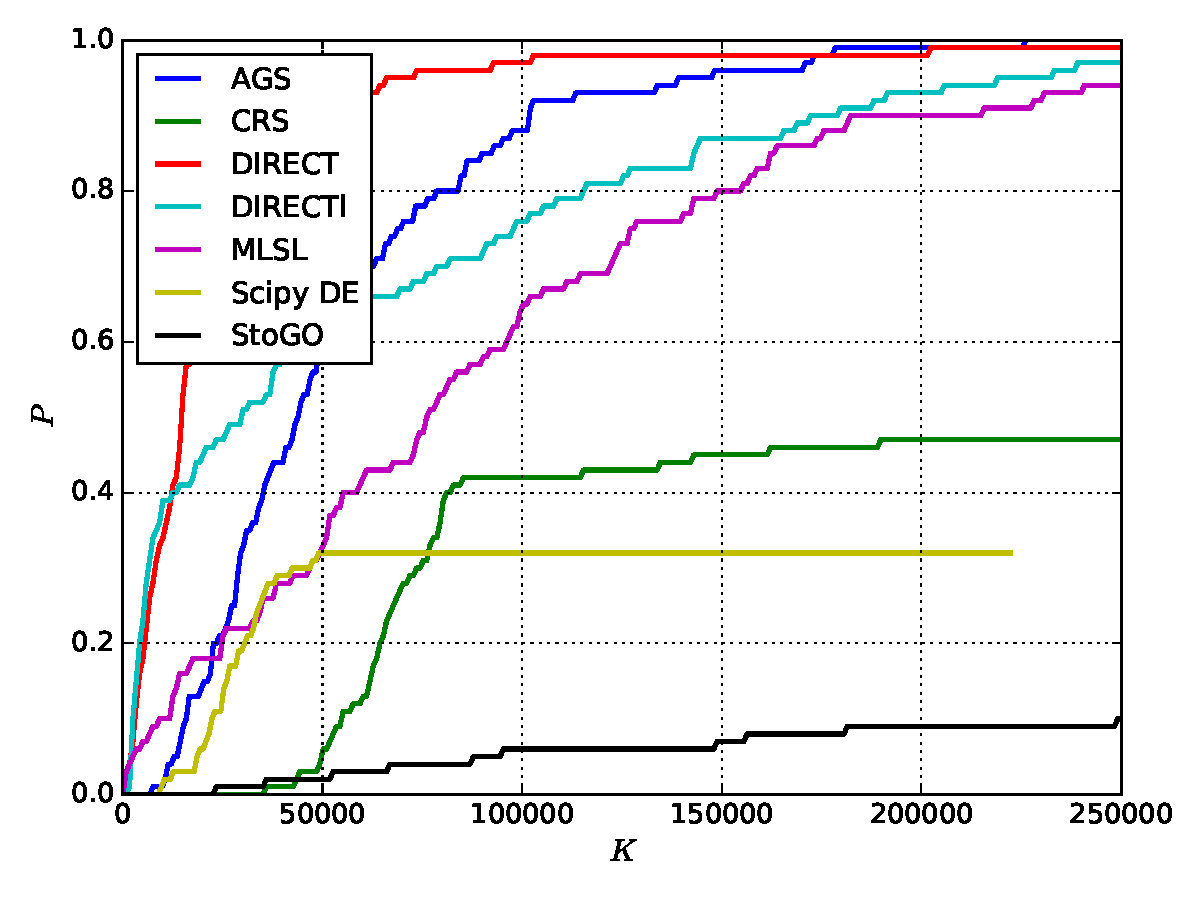
\includegraphics[width=0.95\textwidth]{../experiments/gklsh4d/cmc.pdf}
  \caption{Класс GKLS Hard 4d. Остановка после попадания в окрестность размера $2\cdot10^{-2}$}
  \label{fig:}
\end{figure}

%table gklsh4d
\begin{tabular}{lrr}
\hline
 Метод    &   Среднее число испытаний &   Решено задач \\
\hline
 AGS      &                  54536.84 &            100 \\
 CRS      &                  73779.32 &             47 \\
 DIRECT   &                  23204.38 &             99 \\
 DIRECTl  &                  54489.92 &             97 \\
 MLSL     &                  80247.19 &             94 \\
 SDA      &                  68815.53 &             72 \\
 Scipy DE &                  27466.06 &             32 \\
 StoGO    &                 109328.10 &             10 \\
\hline
\end{tabular}
\begin{figure}[H]
  \center
  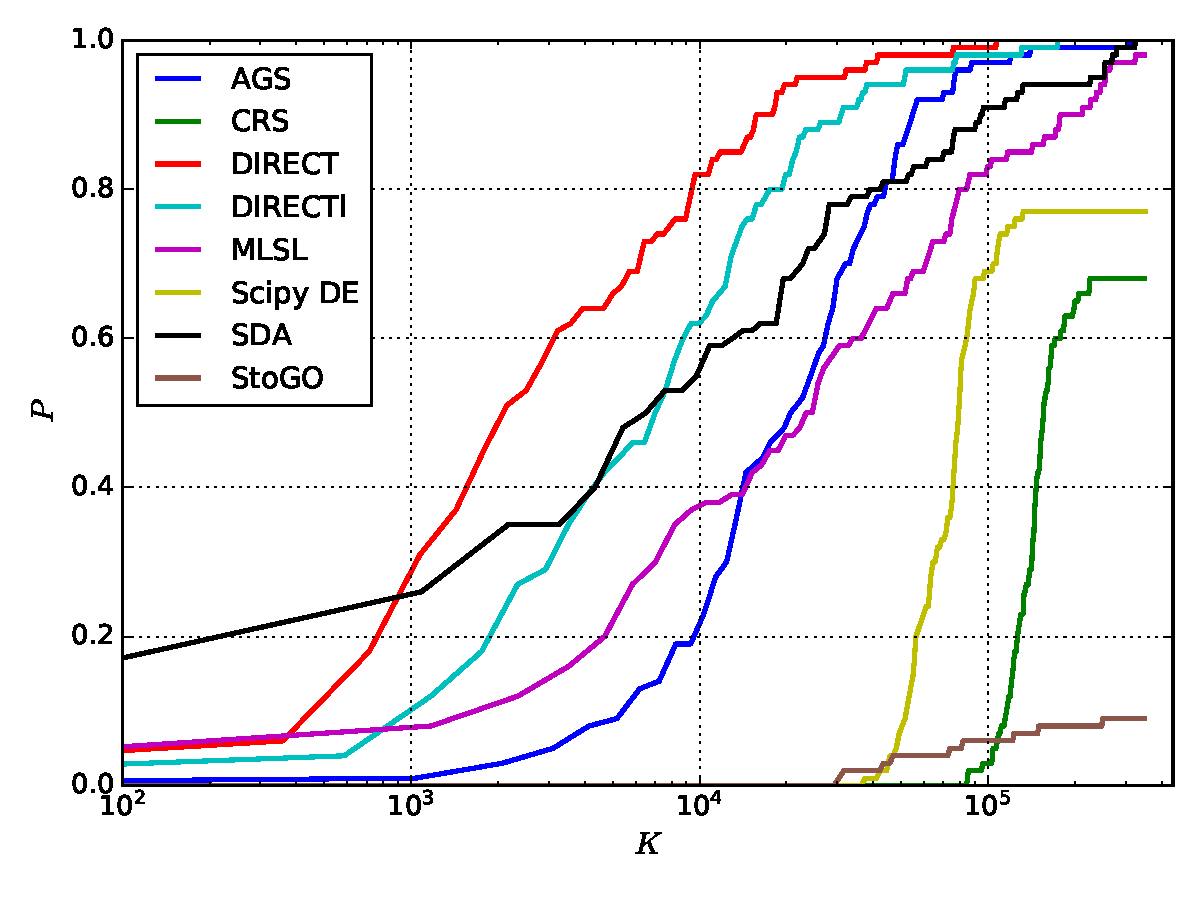
\includegraphics[width=0.95\textwidth]{../experiments/gklss5d/cmc.pdf}
  \caption{Класс GKLS Simple 5d. Остановка после попадания в окрестность размера $2\cdot10^{-2}$}
  \label{fig:}
\end{figure}

%table gklss5d
\begin{tabular}{lrr}
\hline
 Метод    &   Среднее число испытаний &   Решено задач \\
\hline
 AGS      &                  29809.99 &            100 \\
 CRS      &                 143574.99 &             68 \\
 DIRECT   &                   7166.49 &            100 \\
 DIRECTl  &                  13970.53 &            100 \\
 MLSL     &                  52647.63 &             98 \\
 SDA      &                  34255.31 &            100 \\
 Scipy DE &                  73074.52 &             77 \\
 StoGO    &                  91580.44 &              9 \\
\hline
\end{tabular}
\begin{figure}[H]
  \center
  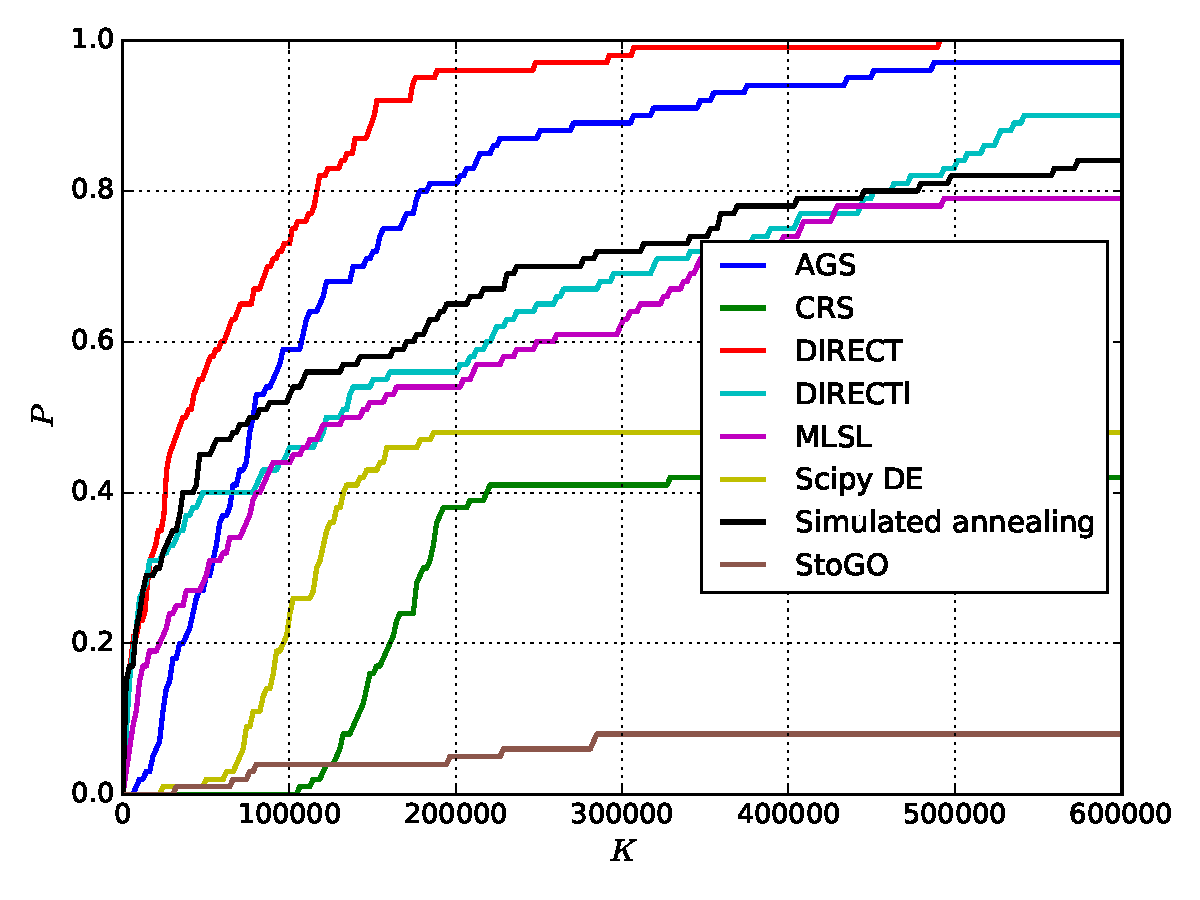
\includegraphics[width=0.95\textwidth]{../experiments/gklsh5d/cmc.pdf}
  \caption{Класс GKLS Hard 5d. Остановка после попадания в окрестность размера $2\cdot10^{-2}$}
  \label{fig:}
\end{figure}

%table gklsh5d
\begin{tabular}{lrr}
\hline
 Метод    &   Среднее число испытаний &   Решено задач \\
\hline
 AGS      &                 113129.08 &             97 \\
 CRS      &                 165192.76 &             42 \\
 DIRECT   &                  66327.42 &            100 \\
 DIRECTl  &                 164390.63 &             90 \\
 MLSL     &                 138766.23 &             79 \\
 SDA      &                 116973.10 &             84 \\
 Scipy DE &                 105496.88 &             48 \\
 StoGO    &                 155123.75 &              8 \\
\hline
\end{tabular}
\begin{figure}[H]
  \center
  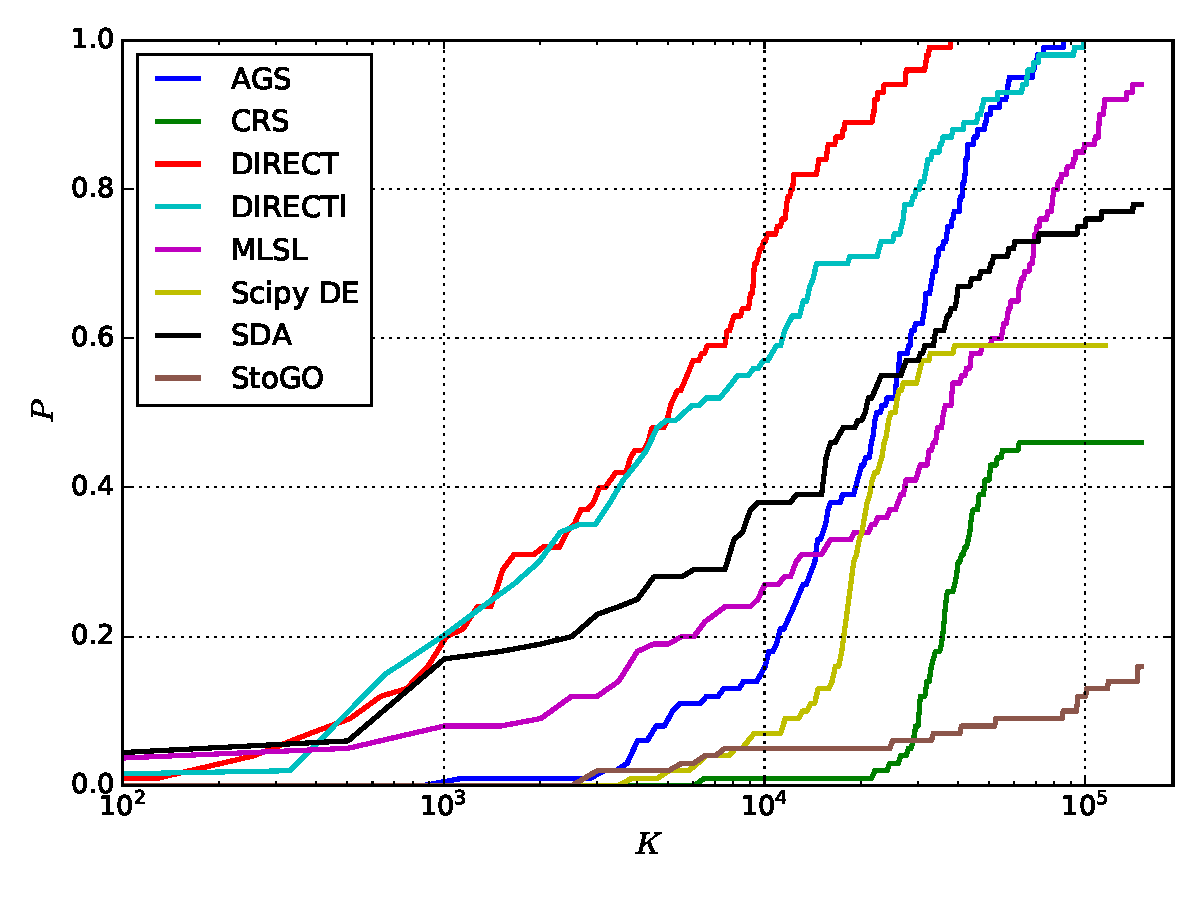
\includegraphics[width=0.95\textwidth]{../experiments/gklss4d/cmc.pdf}
  \caption{Класс GKLS Simple 4d. Остановка после попадания в окрестность размера $0.0632$}
  \label{fig:}
\end{figure}

%table gklss4d_serg
\begin{tabular}{lrr}
\hline
 Метод    &   Среднее число испытаний &   Решено задач \\
\hline
 AGS      &                   5729.82 &            100 \\
 CRS      &                  19883.59 &             74 \\
 DIRECT   &                   7328.78 &            100 \\
 DIRECTl  &                  15010.01 &            100 \\
 MLSL     &                  41484.80 &             94 \\
 SDA      &                  22065.96 &             82 \\
 Scipy DE &                   6271.24 &             68 \\
 StoGO    &                  29359.22 &             72 \\
\hline
\end{tabular}
\begin{figure}[H]
  \center
  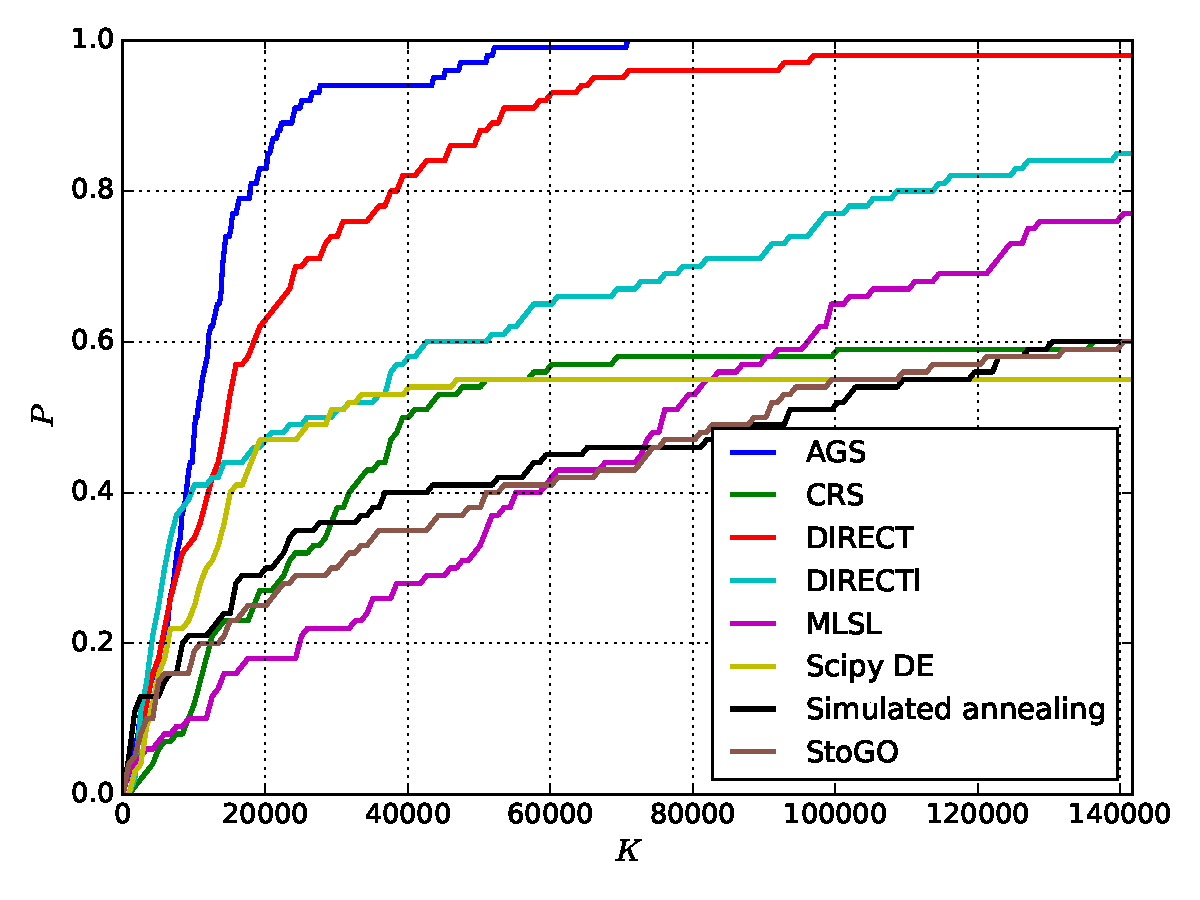
\includegraphics[width=0.95\textwidth]{../experiments/gklsh4d_serg/cmc.pdf}
  \caption{Класс GKLS Hard 4d. Остановка после попадания в окрестность размера $0.0632$}
  \label{fig:}
\end{figure}

%table gklsh4d_serg
\begin{tabular}{lrr}
\hline
 Метод    &   Среднее число испытаний &   Решено задач \\
\hline
 AGS      &                  13113.40 &            100 \\
 CRS      &                  27137.40 &             60 \\
 DIRECT   &                  22884.35 &             99 \\
 DIRECTl  &                  55596.07 &             99 \\
 MLSL     &                  80220.11 &             94 \\
 SDA      &                  68048.01 &             73 \\
 Scipy DE &                  12487.64 &             55 \\
 StoGO    &                  58925.54 &             69 \\
\hline
\end{tabular}
\begin{figure}[H]
  \center
  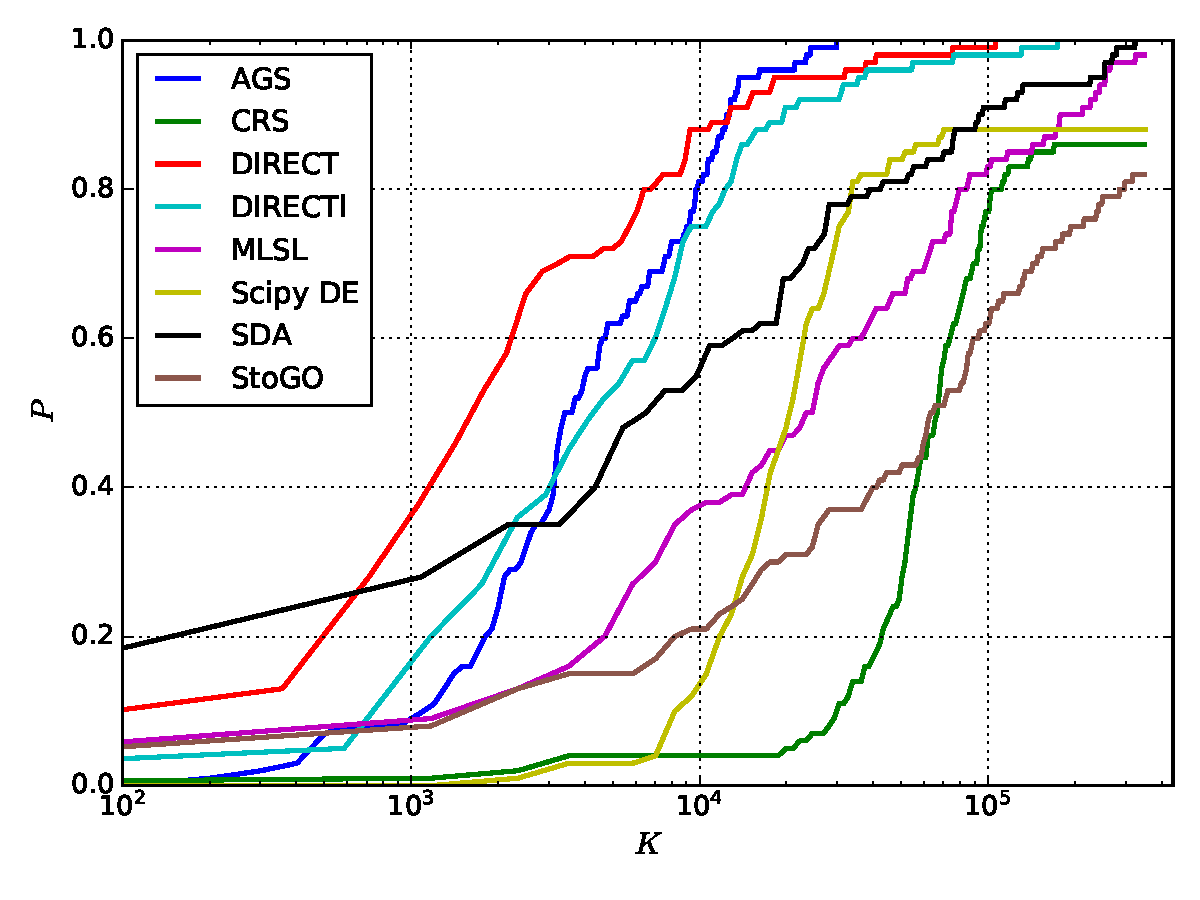
\includegraphics[width=0.95\textwidth]{../experiments/gklss5d_serg/cmc.pdf}
  \caption{Класс GKLS Simple 5d. Остановка после попадания в окрестность размера $0.0796$}
  \label{fig:}
\end{figure}

%table gklss5d_serg
\begin{tabular}{lrr}
\hline
 Метод    &   Среднее число испытаний &   Решено задач \\
\hline
 AGS      &                   5821.47 &            100 \\
 CRS      &                  62921.69 &             86 \\
 DIRECT   &                   5966.13 &            100 \\
 DIRECTl  &                  10795.46 &            100 \\
 MLSL     &                  52609.18 &             98 \\
 SDA      &                  34208.83 &            100 \\
 Scipy DE &                  20859.38 &             88 \\
 StoGO    &                  69206.76 &             82 \\
\hline
\end{tabular}
\begin{figure}[H]
  \center
  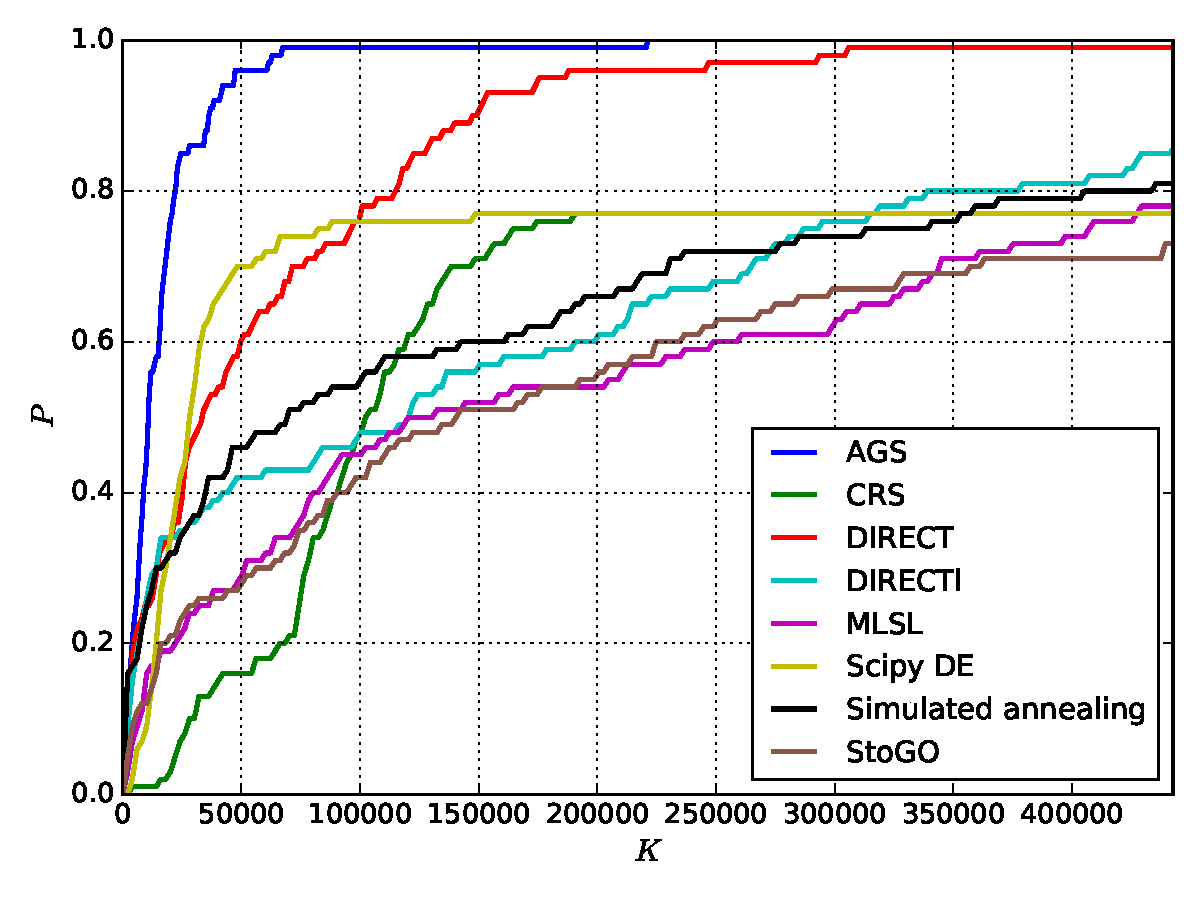
\includegraphics[width=0.95\textwidth]{../experiments/gklsh5d_serg/cmc.pdf}
  \caption{Класс GKLS Hard 5d. Остановка после попадания в окрестность размера $0.0796$}
  \label{fig:}
\end{figure}

%table gklsh5d_serg
\begin{tabular}{lrr}
\hline
 Метод    &   Среднее число испытаний &   Решено задач \\
\hline
 AGS      &                  17008.61 &            100 \\
 CRS      &                  87563.88 &             77 \\
 DIRECT   &                  61657.32 &            100 \\
 DIRECTl  &                 148637.82 &             93 \\
 MLSL     &                 138011.78 &             79 \\
 SDA      &                 115634.59 &             86 \\
 Scipy DE &                  26850.04 &             77 \\
 StoGO    &                 141886.49 &             78 \\
\hline
\end{tabular}
\end{document}
